\documentclass[journal,twocolumn]{IEEEtran}
% documentclass[journal, twocolumn]{IEEEtran}
\usepackage{amsfonts}
\usepackage{amsmath,amssymb}
\usepackage{acronym}  % make an acronym
\usepackage{algorithm}
\usepackage{algorithmic}
% \usepackage{balance}
\usepackage{bm}
\usepackage{bbm}
\usepackage{booktabs}
\usepackage{color, soul}
\usepackage{cite}
% \usepackage{flushend}	% Kunzan leads to problems. 
\usepackage{graphicx}
\usepackage{indentfirst}
\usepackage{lipsum}
\usepackage{setspace}
\usepackage{tikz}
\usetikzlibrary{arrows}
\usepackage{subfigure}
\usepackage[amsmath,thmmarks]{ntheorem}
\usepackage{theorem}
% Enable Hyper-references.
\usepackage{hyperref}
\hypersetup{hidelinks, 
colorlinks=true,
allcolors=black,
pdfstartview=Fit,
breaklinks=true}

\def \H {^H}
\def \opt {^{\text{opt}}}
\def \v {\bm v}
\def \w {\bm w}
\def \g {\bm g}
\def \f {\bm f}
\def \T {\bm \Theta}
\def \t {\bm \theta}
\def \x {\bm \xi}
\def \Pmax {P_{\text{max}}}
\def \ml {multi-layer }
\def \tb {transmit beamformer }
\def \sl {single-layer }
\def \diag {\text{diag}}
\def \opt {^{\text{opt}}}
\def \exp {\text{exp}}
\def \arg {\text{arg}}
\def \CN {\mathcal{CN}}
\def \VM {\mathcal{VM}}
\def \re {\text{Re}}
\def \nc {\mathcal{NC}}
\newcommand{\red}[1]{\textcolor{red}{#1}}
\newcommand{\blue}[1]{\textcolor{blue}{#1}}

\begin{document}

\title{Electromagnetic Information Theory: Fundamentals, Modeling, Applications, and Open Problems}

% \author{{Jieao~Zhu, Zhongzhichao~Wan, and Linglong~Dai, {\textit{Fellow, IEEE}}
% }
\author{{Jieao~Zhu, Zhongzhichao~Wan, and Linglong~Dai, {\textit{Fellow, IEEE}}}
\thanks{J. Zhu, Z. Wan, and L. Dai are with the Beijing National Research Center for Information Science and Technology (BNRist) as well as the Department of Electronic Engineering, Tsinghua University, Beijing 100084, China (e-mails: \{zja21, wzzc20\}@mails.tsinghua.edu.cn, daill@tsinghua.edu.cn).

This work was supported by the National Key Research and Development Program of China (Grant No.2020YFB1807201). }
}

\maketitle

\begin{abstract}
	Traditional MIMO information theory adopts a spatially discrete modeling, which mismatches the continuous nature of the underlying electromagnetic (EM) fields.
	Thus, discrete analysis may fail to reveal the fundamental information transmission limit of a continuous wireless system.    
 	Therefore, it is essential to analyze the information-carrying capability of continuous EM fields, which motivates the research on EM information theory (EIT). In this article, we systematically investigate the basics and the results of EIT. First, we review the fundamental analysis tools of classical information theory and EM theory. Then, we introduce the main research contents in the literature and the corresponding results of EIT, including the continuous field modeling, degree of freedom (DoF), mutual information, and capacity analyses. After summarizing the theoretical analyses, we introduce several applications of EIT to show its guidance to practical systems. Finally, we point out several open problems in EIT, where further efforts are needed to improve EIT towards a unified interdisciplinary theory.
\end{abstract}

\begin{IEEEkeywords}
    Electromagnetic information theory (EIT), channel capacity, Maxwell's equations, prolate spheroidal wave functions (PSWFs). 
\end{IEEEkeywords}

\section{Introduction}
%% leading paragraph. 
Existing wireless theory models transceivers as spatially discrete points. For example, single-input single-output (SISO) theory considers single points as the transceivers, and MIMO theory~\cite{goldsmith2003capacity} utilize discrete point sets in the spatial region to represent the transceivers. 
There have been abundant works on spatially discrete theories and the corresponding MIMO systems. 
However, this discreteness mismatches the spatially continuous electromagnetic (EM) fields~\cite{huang2020holographic}, which are the physical carriers~\cite{migliore2018horse} of information in wireless systems. 
This mismatch may cause a performance gap between the discrete system and the ideal continuous system which suits the EM field. 
Therefore, a theory that can model and analyze the wireless information system with continuous EM fields is necessary, which leads to the research on EM information theory (EIT).

EIT is an interdisciplinary subject that integrates deterministic physical theory and statistical mathematical theory to study the transmission mechanism of information in the spatially continuous EM field. 
Specifically, EIT unites the basic laws and methodologies in both the classical EM theory and the information theory. 
As a result, EIT is capable of building the system modeling and performance analysis frameworks that fit the EM propagation theory for wireless information systems. 

%% Our contributions.
In this article, we systematically investigate the analysis techniques and the corresponding results of EIT. The key features of this article can be summarized as follows:
\begin{itemize}
\item{The fundamental mathematical tools in classical information theory and EM theory are briefly reviewed. Specifically, the degrees of freedom (DoF), prolate spheroidal wave functions (PSWFs), channel capacity, and Maxwell's equations are firstly introduced. To integrate the probabilistic nature of information theory and the continuous property of EM fields, random fields are then introduced as a core EIT concept, which enables the EIT performance analysis. }
\item{The basic EIT modeling methodologies are introduced for both the EM channels and the EM noise. For EIT channel modeling, both the deterministic and stochastic modeling approaches are discussed. For EIT noise modeling, the noise fields are first categorized according to their different physical origins, and then the spatial correlation characteristics of different kinds of noise fields are discussed separately. }
\item{The theoretical EIT peformance analysis methods are introduced. By applying the EIT modeling methodologies, the DoF, mutual information, and capacity can all be derived by mathematical tools including the PSWFs, Karhunen-Lo\`{e}ve expansion, and random field theories. } 
\item Moreover, several EIT-related applications are introduced, in which they are guided by the EIT performance analysis. To approach the EIT capacity, the continuous aperture MIMO (CAP-MIMO) has been proposed to fully harvest mutual information in a limited aperture area. To fully exploit the distance-domain DoF predicted by EIT, the location division multiple access (LDMA) technology has been proposed to utilize extra spatial resources to serve users. In addition, a distance-aware precoding (DAP) scheme has been proposed to take advantage of the extra channel DoF in the near-field region.  % Other applications include precise field extrapolation and reconstruction based on the statistical characteristics provided by EIT modeling. 
\item{Finally, several open problems in EIT are pointed out, involving the compatible noise modeling, the physically appropriate power constraint, the achievability of the EM capacity, and the physical granuarity limit of current manipulation.}
\end{itemize}

\section{Fundamentals}
In this section, we first distinguish between two different definitions of DoF in information theory, where PSWFs are introduced as basic analytical tools to obtain the DoF. 
Then, we clarify the concept of channel capacity and its relation to DoF. 
After that, we introduce Maxwell's equations to describe information transmission via EM fields. 
Finally, we employ random fields as the EIT foundation for unifying the probabilistic information theory and deterministic field theory. 

% In this section, we will first brief on the fundamental building blocks of the classical one-dimensional time-domain information theory in Subsection~\ref{Sec_2_Subsec_1}. 
% Then, the four-dimensional electromagnetic basics for wireless communications are introduced in Subsection~\ref{Sec_2_Subsec_2}. Finally, two different approaches of combining the information theory with the electromagnetic theory are discussed. 

\subsection{Degrees of Freedom}
\label{Sec_2_Subsec_1}
% introduce the channel DoF. 
DoF is a mathematical quantity that describes the number of independent parameters in a physical system. 
Usually, in the communication context, the DoF refers to the number of orthogonal subchannels that can carry information independently, which is uniquely determined by the channel characteristics and calculated by counting the significant singular values of a given channel matrix \cite{goldsmith2003capacity}. 
Thus, we use the term {{\emph{channel DoF}}} to describe such a number associated with a channel.



% introduce the functional DoF. The formulas 2WT+o(2WT) is indispensable here. 
In contrast, the DoF is defined asymptotically in the information theory context. From a rigorous point of view, the (asymptotic) DoF is defined to be the minimum dimension of a finite-dimensional functional subspace that can approximate any function in a larger space with arbitrarily small error~\cite{poon2005degrees}. For example, the DoF of $W$-bandlimited signals with observation duration $T$ can be derived by finding the finite-dimensional subspace which contains all the $W$-bandlimited functions that are most concentrated in the time domain. The problem of finding these most concentrated functions is named Slepian's concentration problem~\cite{slepian1976bandwidth}, and it has explicit solutions called PSWFs, as is shown in Fig.~\ref{fig:PSWF}.
More interestingly, it is proved that to approximately represent any $W$-bandlimited function, it suffices to pick out $2WT+o(2WT)$ PSWFs as basis functions. Thus, the functional DoF of the $W$-bandlimited signals is $2WT+o(2WT)$ \cite{slepian1976bandwidth}. 
Since this kind of DoF numerically characterizes the possibility to approximate a generally infinite-dimensional functional space by a finite-dimensional subspace, we refer to it as the {{\emph{functional DoF}}}. 
It is worth noting that the functional DoF can be alternatively interpreted as the number of minimal required samples to approximately reconstruct an unknown signal. 
\begin{figure}
	\centering 
	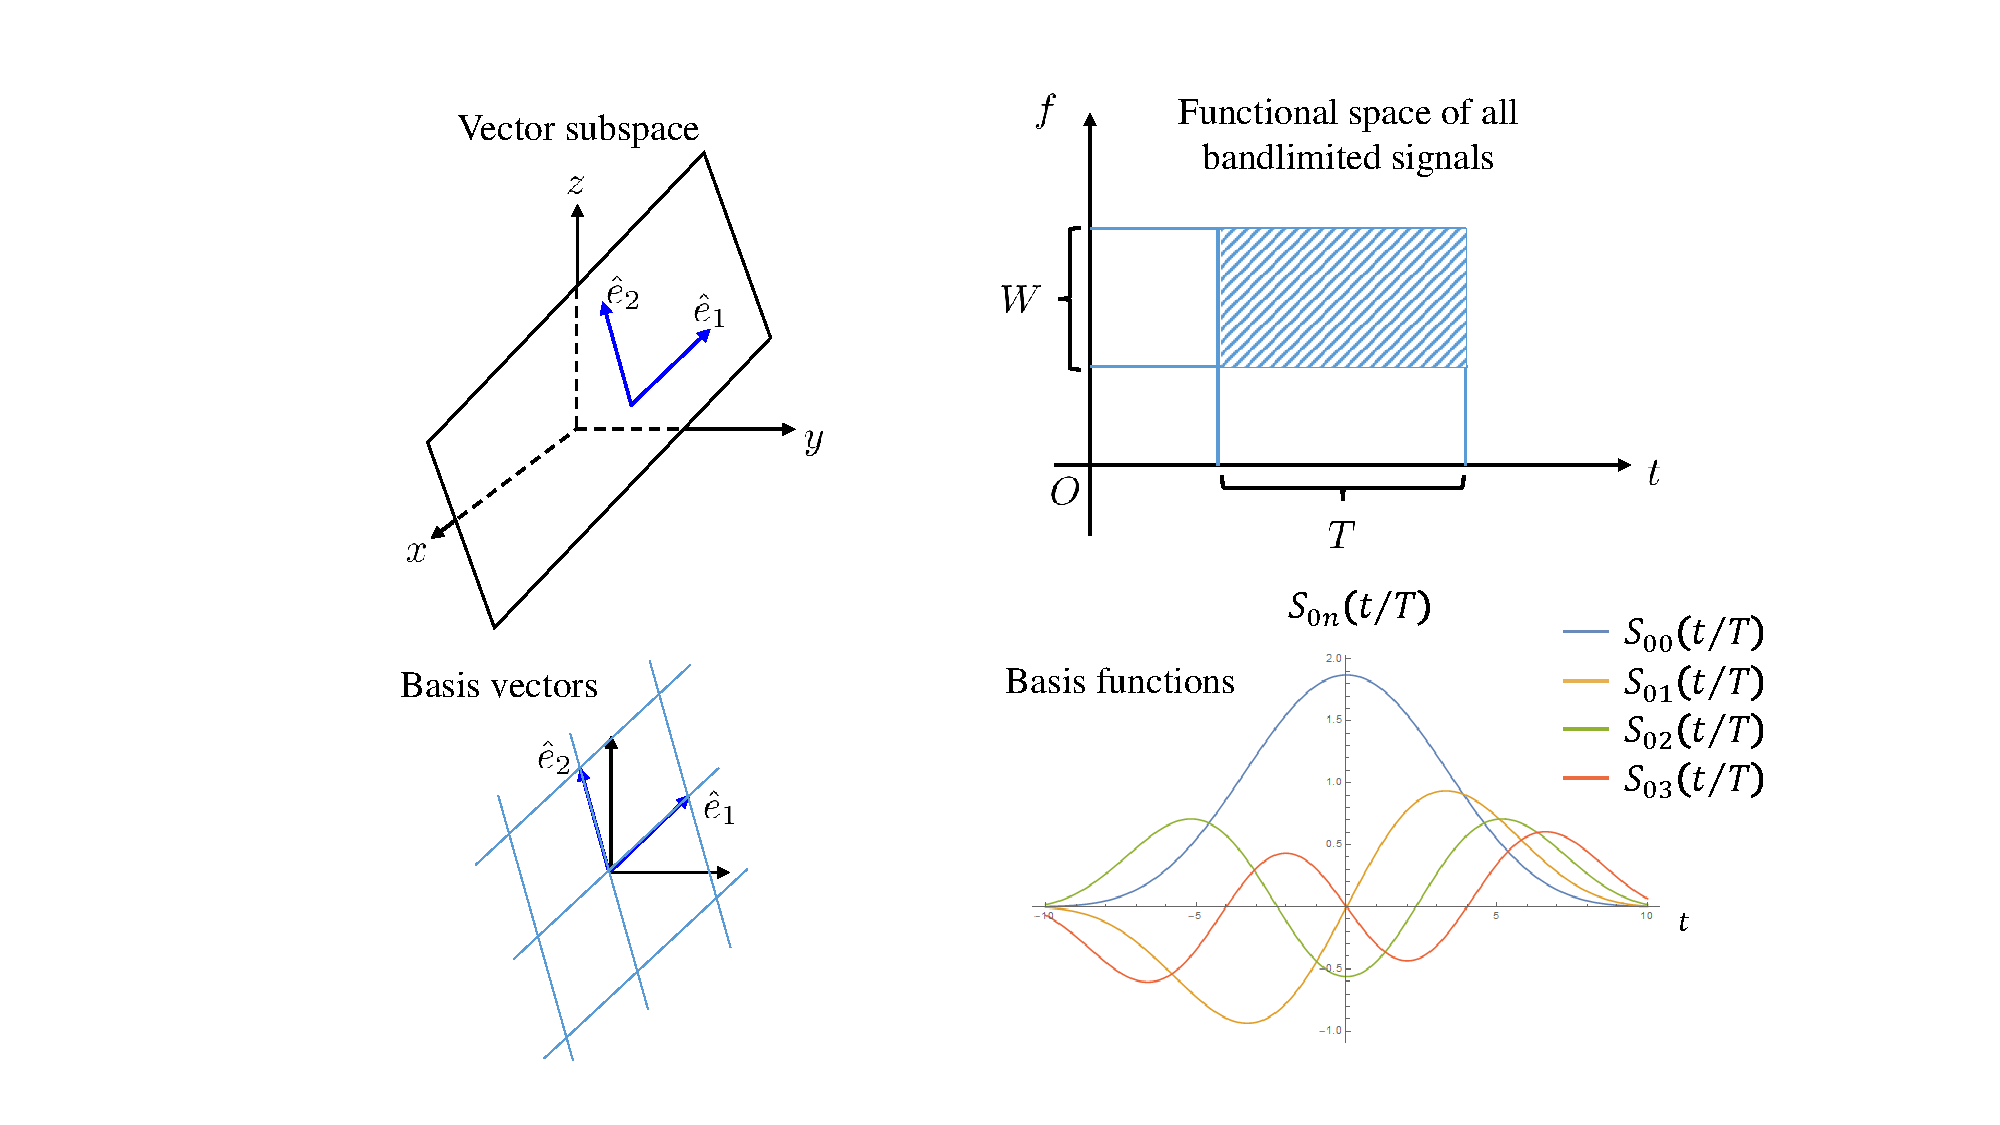
\includegraphics[width=\linewidth]{figures/PSWF.pdf} 
	\caption{Illustration of functional spaces and their analogy with finite-dimensional vector spaces. The basis of the functional space is portrayed by PSWFs. }
	\label{fig:PSWF}
\end{figure}

% introduce PSWF and its connection to the evaluation of functional DoF. 
% The explicit evaluation of the functional DoF of arbitrary given functional space is hard in general. However, in some special but important cases this task can be fulfilled by leveraging the constraints that define the functional space.
% For example, the functional space $\mathcal{B}_W$ that contains all the $W$-bandlimited functions can be decomposed by finding those particular bandlimited functions that are most concentrated in the time domain. The problem of finding these most concentrated functions, which is named as Slepian's concentration problem, has explicit solutions called PSWFs.
% More interestingly, it is proved that in order to approximately represent any function in $\mathcal{B}_W$, it suffices to pick out $2WT+o(2WT)$ PSWFs as basis functions. Thus, the functional DoF of $\mathcal{B}_W$ is $2WT+o(2WT)$. 

% Similar to the singular decomposition method for evaluating the channel DoF, the functional DoF of a given signal space is evaluated by approximating the signal space by a finite-dimensional subspace. In the case of band-limited functional space, this decomposition where the basis functions of the subspace are obtained by solving a the Slepian's concentration problem, and the solutions are proved to be the prolate spheroidal wave functions (PSWFs). 

\subsection{Channel Capacity}
\label{Sec_2_Subsec_2}
Different from the notion of channel DoF which characterizes the number of orthogonal subchannels available, the channel capacity measures the error-free information transmission capability of the channel. 
Since the transmission errors are caused by random channel noise, the channel is information-theoretically defined to be a conditional transition probability that maps the channel input randomly to the output. 
Then, the mutual information between the input and output can be defined, and the channel capacity is derived by taking the supremum of the mutual information over all the input distributions of the channel. 

The operational meaning of the channel capacity is established by Shannon in his seminal paper~\cite{shannon1948mathematical}. To establish the operational meaning, he proved the achievability and ``converse'' theorem of the channel capacity. The achievability means that, for any given error probability and code rate lower than the capacity, there exists a pair of encoder-decoder of sufficient code length to operate below such error probability. 
The ``converse'' theorem means that for an arbitrary code rate higher than capacity, no matter what code is employed, the error probability is bounded away from zero. This result indicates that it is impossible to realize error-free transmission if transmitting at a higher-than-capacity rate. Thus, the value of channel capacity is established to be the fundamental transmission limit of such a given channel. 
%% (TODO) Add the relationship between the DoF and the channel capacity. 

% The second step is to discretize the continuous time-domain waveform channel into a series of independent symbol channels, and sum over the capacities of each symbol channel to obtain the overall waveform channel capacity. Without loss of generality, a $W$-bandlimited waveform channel is first considered, which is equivalent to setting $h(t)=W{\rm sinc}(Wt)$. Not rigorously, this discretization step is done by the Shannon-Nyquist sampling theorem, stating that a number of $2WT$ independent samples can be obtained from a waveform channel bandlimited to $W$ and time-limited to $T$. From a more rigorous functional point of view, the $W$-bandlimited waveform channel is viewed as a projection operator $\mathcal{B}$ that maps a signal $x\in{\mathcal{L}^2(\mathbb{R})}$ into the bandlimited received signal $y={\mathcal{B}x}$, and the information-transmission capability of such operator $\mathcal{B}$ is characterized by its eigenvalues over a finite time interval $[-T/2, T/2]$. This eigenproblem is referred as the Slepian's concentration problem. Solving this eigenproblem directly leads to the eigenfunctions called prolate spheroidal wave functions (PSWF), and the number of significant eigenvalues above a certain threshold is exactly $2WT+\mathcal{O}(\log(WT))$. The number of these dominating eigenvalues are often referred to as the degrees of freedom (DoF) of this channel, which means that this $W$-bandlimited $T$-timelimited waveform channel can be asymptotically viewed as $2WT$ parallel Gaussian symbol channels, as $T\to\infty$. The capacity of a $W$-bandlimited channel, in bits per second, can then be derived accordingly. 

% The third step is to integrate over the frequency axis to get the overall capacity, exploiting the capacity result of a $W$-bandlimited waveform channel. Specifically, for any given small frequency band $[f, f+{\rm d}f]$, the capacity of such infinitesimal sub-channel is jointly determined by the frequency response $|H(j2\pi f)|^2$ of $h(t)$, the AWGN noise level, and the power budget\footnote{The power budget of the transmitted signal $x(t)$ is usually characterized by the power spectral density (PSD) $S_x(f)$, where $f$ varies within the bandwidth of the wireless system in question. } of transmitted signal $S_x(f)$ at single frequency point $f$. Thus, integrating over the entire frequency axis yields a capacity value of the AWGN waveform channel with impulse response $h(t)$. The achievability and converse of such a capacity is guaranteed by performing asymptotic error analysis on all the above three deduction steps. 

\subsection{Electromagnetic Theory}
\label{Sec_2_Subsec_3}
% Basics about electromagnetics.
EM theory plays a cornerstone role in designing wireless systems. Specifically, EM theory is a branch of physics that studies the EM interaction in four-dimensional spacetime from a field-theoretic point of view. The EM forces are carried by EM vector fields, which are usually described by Maxwell's equations. Maxwell's equations are four linear partial differential equations that characterize how the electric fields and magnetic fields are altered by each other and by charges and currents. Combining these four equations, a vector wave equation can be obtained that manifests the existence of EM waves. 
\begin{figure}
	\centering 
	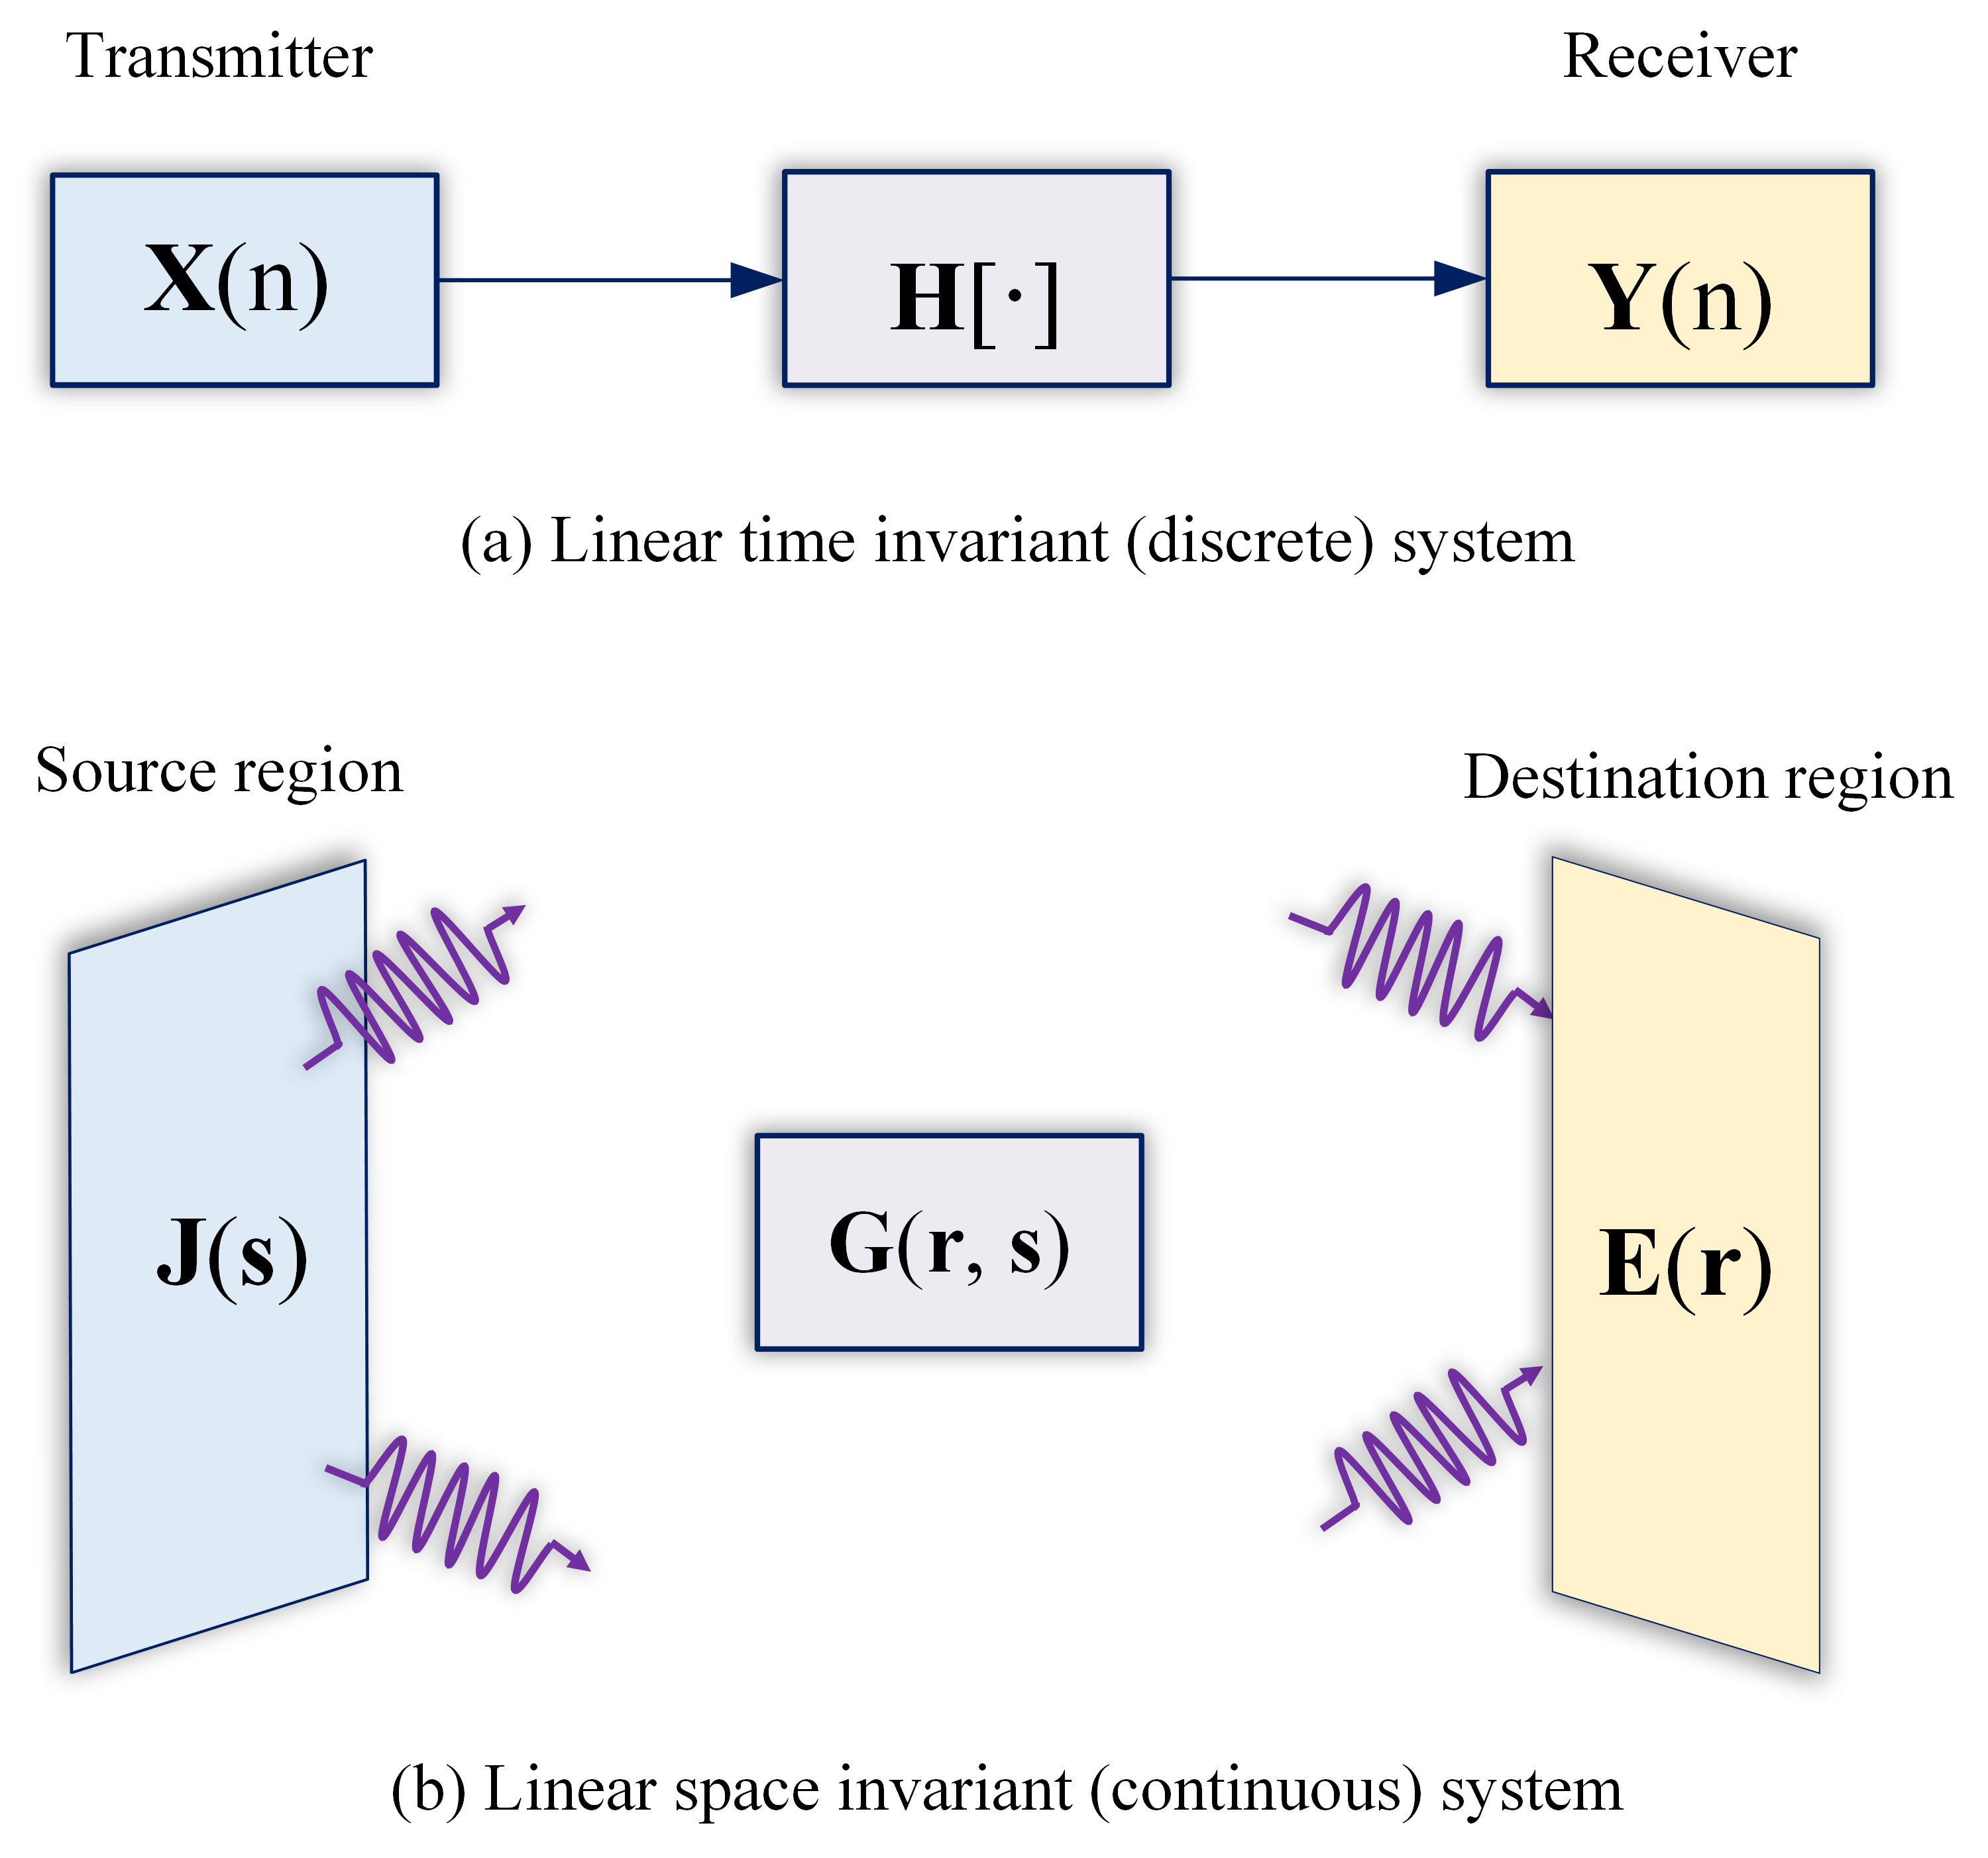
\includegraphics[%height=4cm,
	width=6.8cm]{figures/Shannon_Marzetta.png} 
	\caption{Linear time invariant systems described by an impulse response in classical information theory, compared with linear space invariant systems described by the Green's function in EIT.} 
	\label{fig:Shannon_Marzetta}
\end{figure}

In wireless communications, in order to describe the EM response at the receiver induced by the transmitted wave at the transmitter, Green's function is often introduced as the spatial impulse response of EM systems~\cite{stratton2007electromagnetic}, as is shown in Fig.~\ref{fig:Shannon_Marzetta}. Since the electric and magnetic field vectors are all three-dimensional time-varying vectors, Green's function is a dyad-valued function of spacetime. 
Note that EM theory is a deterministic theory built on partial differential equations and the knowledge of all the surroundings, and thus Green's function is uniquely determined by the boundary conditions of EM problems.
As a result, pure EM theory cannot capture the random nature that arises in communications. 

\subsection{Random Fields for EIT}
\label{Sec_2_Subsec_4}
In order to apply information-theoretic analysis to EM fields, probabilistic measures should be assigned to the functional space containing all the possible EM fields that satisfy Maxwell's equations, which leads to the random field modeling for EIT. 
Random fields are well-studied mathematical objects, among which the Gaussian random fields (GRFs) are the most widely applied instances. 

GRFs are random multivariate functions whose finite-dimensional marginal distributions are Gaussian. Justified by the central limit theorem, many complicated spatially dependent random values that arise in communications can be modeled by GRFs.  
Inheriting favorable mathematical properties from Gaussian distributions, such GRF modeling exhibits good analytical properties that can facilitate both theoretical deduction and numerical inference. 

In EIT, the GRFs can be utilized to model both the EM channels~\cite{marzetta2022fourier} and the EM signals~\cite{wan2022mutual}. Since in real-world communication scenarios the EM channel responses vary randomly as a function of spacetime, it is reasonable to model such spatio-temporal variations by a channel GRF, thus allowing Bayesian inference of the channel entries that are not directly measured. 
Similarly, in order to capture the randomness of the transmitted and received signals, the current distributions at the transmitter and the electric fields at the receiver can also be modeled by GRFs~\cite{wan2022mutual}, from which information-theoretic mutual information can be defined to characterize the information transmission capability of such EM channels. 


% Motivated by the possibility of exploiting the three spatial dimensions, the multi-input multi-output (MIMO) architecture have been ubiquitous in contemporary wireless communication systems. To fully exploit the potential of MIMO, numerous spatial multiplexing technologies have been proposed, including SDMA, TRDMA, PDMA, and LDMA. However, there must be a unified underlying theory that governs all the multiplexing technologies, since they are all based on the same physical media of electromagnetic waves. To construct this unified theory, two different approaches have been proposed in the literature to characterize the electromagnetic channel. 

% The first approach is to model the electromagnetic channel in a deterministic manner. The determination of the modeling means the channel is treated as a fully predictable function of spacetime, as long as the geometric parameters of the transceivers and the scatterers are known. A typical modeling of such a deterministic channel is describing the electromagnetic channel with the dyadic Green's function. The dyadic Green's function, which can be directly derived by solving the vector wave equation of electromagnetic fields, can be regarded as the spatial impulse response of the electromagnetic field with given boundary conditions. Similar to the decomposition of a $W$-bandlimited time-domain waveform channel, the four-dimensional electromagnetic channel, described by some deterministic Green's function, can be decomposed onto a certain orthonormal eigenfunctions, and the corresponding eigenvalue set determines all the information-theoretic numerical characteristics of such channel, including the DoF and capacity.

% The second approach is to model the electromagnetic channel in a stochastic manner. Instead of treating the electromagnetic channel by some deterministic impulse response, this stochastic modeling regards the channel itself as a random field, in which the electromagnetic constraints brought by Maxwell's equations are encoded in the auto-correlation function of such a random field. By this approach, we can obtain the ergodic capacity, but the exact DoF cannot be defined with such a stochastic assumption.  


% In wireless communications, electromagnetic waves are often exploited to carry information by manipulating their amplitudes, frequencies, and phases. To transmit and receive the electromagnetic waves, antennas are designed to radiate the waves into the free space at the transmitter, and couple the waves into electronic circuits at the receiver. Thus, from an end-to-end point of view, by applying antennas, the electromagnetic channel in four-dimensional spacetime is simplified into a time-domain waveform channel with only one temporal dimension. 
% In this simplified model, both the electromagnetic properties of the propagation environment and the detailed design of the antennas are condensed into an end-to-end impulse response $h(t)$ of the time-domain equivalent channel, to which Shannon's information-theoretic approach in the previous Subsection~\ref{Sec_2_Subsec_1} can then be applied. 
% It is worth noting that, with this end-to-end single-input single-output (SISO) model, only one time dimension out of four spacetime dimensions of the electromagnetic waves can be efficiently utilized. Thus, the DoF of the electromagnetic channel is well under-exploited in SISO technology. 


\section{Modeling Methodologies in EIT}
In this section, we first discuss the continuous modeling scheme in EIT, which contains both the channel modeling and the noise field modeling. 
Based on the continuous modeling of the system, we further utilize tools in information theory like PSWF to derive the DoF, mutual information, and capacity.

\subsection{Continuous channel modeling}
In this part, we will discuss the channel models in EIT, which describes the EM channel by a linear transformation from the radiated field to the noiseless received field.  
% Since spatial multiplexing can only be realized with MIMO technology, we will always assume a MIMO transceiver in the sequel. 
Note that to model a traditional narrowband MIMO channel, a matrix with complex-valued entries is usually utilized, each representing the complex channel gain between a pair of transceiver antennas. 
This channel model is, in essence, spatially discrete. 
However, in EIT, it is reasonably assumed that one can measure the field at an arbitrary point inside the receiver region, where the precision of such measurement is subject to some physical noise limits. This leads to the assumption of EIT that the transceivers operate in a continuum of space.  

This idea of continuous modeling, though seems impossible to have its hardware correspondence in reality, is of both theoretical convenience and practical reasons. 
The theoretical convenience originates from the fact that the fundamental physical laws that rule the EM phenomena are intrinsically continuous. 
As a result, extensive mathematical tools, including functional analysis, linear operator theory, and complex analysis, have already been developed to tackle these continuous linear problems. 
The practical reasons are that the real-world antenna-based point-to-point transmission models can be viewed as a special case of the continuous model. 
Mathematically, an antenna acts as a continuous integral operator that weights the incident signal by its EM eigenmode, which corresponds with the continuous modeling in EIT. 
Thus, the EIT channel model is expected to be written in a continuous linear operator language, whether the operator is deterministic or stochastic.

For the deterministic channel modeling approach, the simplest channel model is the line-of-sight (LoS) model, which assumes no scatterers between the transceivers. In this scenario, the channel operator is the free-space Green's function. More complex modeling schemes consider the scatterers and group them into clusters. The channel operator is thus dependent on the locations of the clusters.

\begin{figure}
	\centering 
	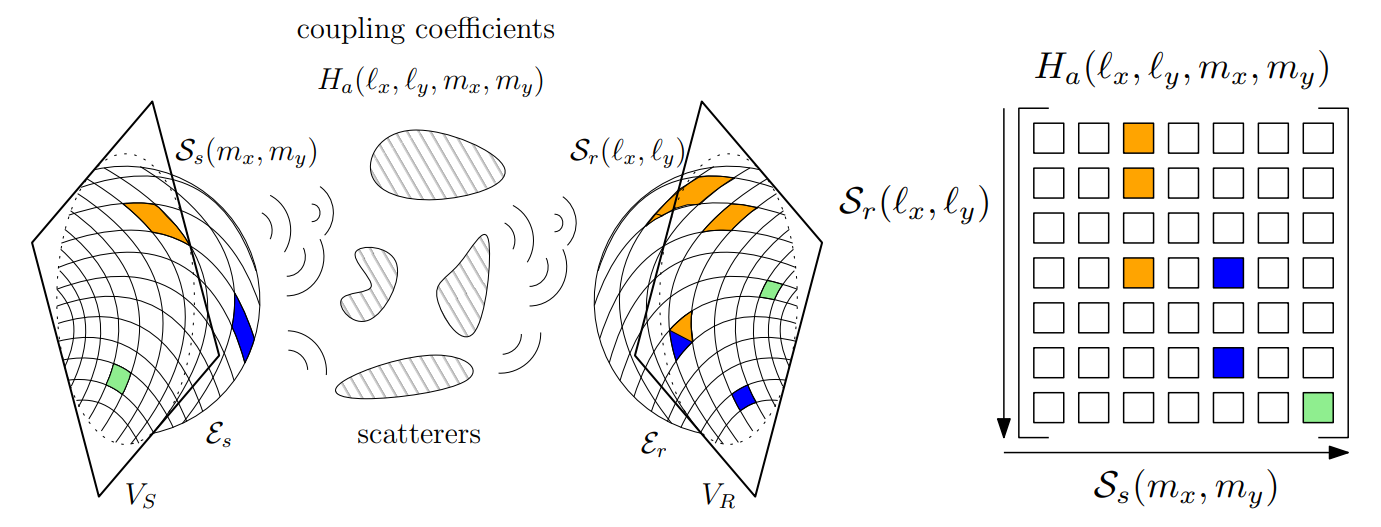
\includegraphics[width=\linewidth]{figures/random_channel.png} 
	\caption{Continuous stochastic channel modeling, where the linear channel operator is projected onto the Fourier plane-wave basis~\cite{marzetta2022fourier}.} 
	\label{fig:marzetta}
\end{figure}
Another modeling approach is the stochastic channel modeling, where some statistical characteristics of the channel are available. As introduced in Subsection~\ref{Sec_2_Subsec_4}, GRFs are suitable to model the randomness of the channel and can provide useful tools such as Bayesian inference for channel estimation. For stochastic channel modeling, a novel method is the Fourier plane-wave expansion which decomposes the channel using plane waves~\cite{marzetta2022fourier}. Such expansion is shown in Fig.~\ref{fig:marzetta}, and it is equivalent to performing Fourier transform on the stochastic channel. The spectrum of the channel in the wavenumber domain and the autocorrelation function of the channel can also be derived under the GRF channel model, which can facilitate the mutual information and capacity analysis of the channel.

\subsection{Noise field modeling}
After the discussion of the continuous random channel models, we will introduce the noise modeling scheme. 
Noise is vital in information theory, because it determines the capacity together with the signal. 
In classical information theory, the noise is usually modeled by a time-domain AWGN, since the AWGN has a flat power spectral density (PSD) and its projection coefficients onto any orthonormal basis are independent and of equal power, which is beneficial to theoretical analysis. 
Similarly, in EIT, the noise is usually modeled as a spatial AWGN with flat wavenumber PSD. This spatial AWGN implies that the additive noises at any small spatial regions are independent and identically distributed (i.i.d) proper complex Gaussian random variables whose variances are proportional to the volume of the small region. This is the simplest noise model in EIT, which is convenient for analysis, but there are still gaps towards reality. 

In general, the noise values that emerge on different points of space cannot be assumed independent, i.e., they do exhibit some spatial correlation. 
This is because the noise is not completely composed of spatially uncorrelated thermal noise. 
The unwanted interference waves wandering in the space also enter the receiver, leading to an equivalent noise signal which is spatially correlated in general. 
To characterize this EM interference, the one-ring model~\cite{patzold2004space} is borrowed from prior works on channel modeling and is extended to a more general one-sphere scenario with polarized EM waves~\cite{wan2022mutual}, while the analytical expressions of the spatial correlation function can still be obtained. 
This non-white spatially correlated noise model is of theoretical importance, since it is provably compatible with Maxwell's equations, while other noise models including the sinc-shaped or jinc-shaped correlation functions fail to satisfy Maxwell's constraints because they ignore the polarization of the EM waves. 

\section{Information-Theoretic Analysis in EIT}
In this section, based on previous discussions about EIT modeling, we introduce the basic performance indicators and the corresponding analysis techniques in EIT, including the functional DoF, the channel DoF, and the capacity. 
% For a wireless system, the DoF shows the maximum number of independent channels that can be utilized to transmit information. For example, the DoF of a traditional MIMO system is usually approximated by the minimum value of the number of transmitting antennas and the number of receiving antennas. However, such approximation fails when we consider massive antennas in a spatially-constraint region, because the approximated DoF will tend to infinity with the growth of the number of antennas. Therefore, the true DoF value of a spatially constrained continuous wireless system is worth analyzing. In this subsection, we will discuss the functional DoF and channel DoF in EIT separately, and summarize the related works.


\subsection{Functional DoF}\label{Sec_4_Subsec_1}
As we have clarified in Section~\ref{Sec_2_Subsec_2}, the functional DoF in classical information theory represents the minimum number of samples that is needed to reconstruct the signal. Similarly, in EIT, the functional DoF refers to the minimum number of samples that is needed to reconstruct a given EM field. 
Such a functional DoF is closely related to the transmission capability of the EM system, because the minimum number required samples to reconstruct an EM field is equivalent to the maximum number of complex values that can be transmitted within a single EM channel use. 

The basic analysis technique of such functional DoF is similar to the application of the Nyquist sampling theorem in classical information theory. 
Similar to the bandlimited signals in the time-frequency domain, the radiated EM fields also exhibit wavenumber-limited property in the space-wavenumber domain. 
Thus, it can be easily proved that a half-wavelength sampling suffices to asymptotically reconstruct an arbitrary EM field, i.e., the EM DoF is at most proportional to the number of half-wavelength grids in the receiver region, given that the receiver region is sufficiently large. 
% If we observe the EM field in a spatially limited region, of which the size is far larger than the wavelength of the EM field, then we can perform half-wavelength sampling on the region. The DoF obtained from the region is asymptotically proportional to its length or area. 

A more refined analysis on the wavenumber-limitedness of the EM fields show that the EM functional DoF depends on how rapid the phase of a radiated field changes over space. 
To describe such phase change, the authors of~\cite{bucci1987spatial} coined the word ``spatial bandwidth'' to characterize the degree of wavenumber-limitedness, where they adopted Laplace's steepest descent method to show the preciseness of such field reconstruction and prove the correctness of the derived functional DoF. 

% In the analysis approach of spatial functional DoF, a notion named spatial bandwidth is introduced, which extends the bandwidth in classical information theory to spatial domain~\cite{bucci1987spatial}. The bandwidth in classical information theory depicts the band-limited characteristics of the signal in the frequency domain, and can be used to derive the DoF of the signal according to the Nyquist sampling theorem. Similarly, the spatial bandwidth depicts the band-limited characteristics of the EM field in the wavenumber domain, and can be used to derive the DoF of the EM field in the space-wavenumber domain. For a given channel model, the spatial bandwidth can be approximated using the method of steepest descent. More general results considering the four-dimensional spacetime are based on Landau's eigenvalue problem.

\subsection{Channel DoF}
The functional DoF introduced in the previous subsection emphasizes the intrinsic DoF of the received field. 
However, it is possible that due to the restrictions of the EM channel, some of these functional DoF at the receiver cannot be excited. For example, an EM propagation environment rich in scatterers can excite almost all the angular eigenmodes at the receiver, while an EM channel composed only of LoS paths may not enable all of the functional DoF. Thus, evaluating the channel DoF is of practical importance.  

As is defined in Subsection~\ref{Sec_2_Subsec_1}, the channel DoF represents the maximum number of independent parallel channels that can be used to transmit information. 
For the simplest line-of-sight (LoS) channel, the DoF is solved by expanding the continuous channel on a series of orthogonal sub-channels and counting the number of channel gains that exceed a threshold. 
This procedure can be transplanted into EIT by solving the eigenvalue problem of the continuous channel operator. 
Specifically, the LoS channel operator is given by the free-space Green's function, and the corresponding eigenvalue problem can be approximated by Slepian's concentration problem~\cite{miller2000communicating}, where the well-investigated PSWFs are the approximated eigenfunctions.  
Through this approach, the DoF of LoS channel model approximately derived to be  proportional to the product of the area of the transceivers~\cite{pizzo2022nyquist,miller2000communicating}. 

For non-line-of-sight (NLoS) channel models where the deterministic scatterers are packed into some known solid angular regions, since the angular domain and the antenna domain are Fourier transform pairs, the channel DoF can be similarly derived by performing Slepian's analysis in the angular domain. It is proved that the NLoS channel DoF is proportional to both the solid angle of the scatterer cluster and the geometric lengths of the transceivers~\cite{poon2005degrees}.  
If the channel is modeled as a stochastic channel with random scatterer positions, uniform distributions or von Mises-Fisher distributions can be used to model the statistical characteristics of the channel. 
The DoF of the channel in this stochastic model should be the expected value averaged by probability.

\begin{figure*}[ht]
	\centering 
	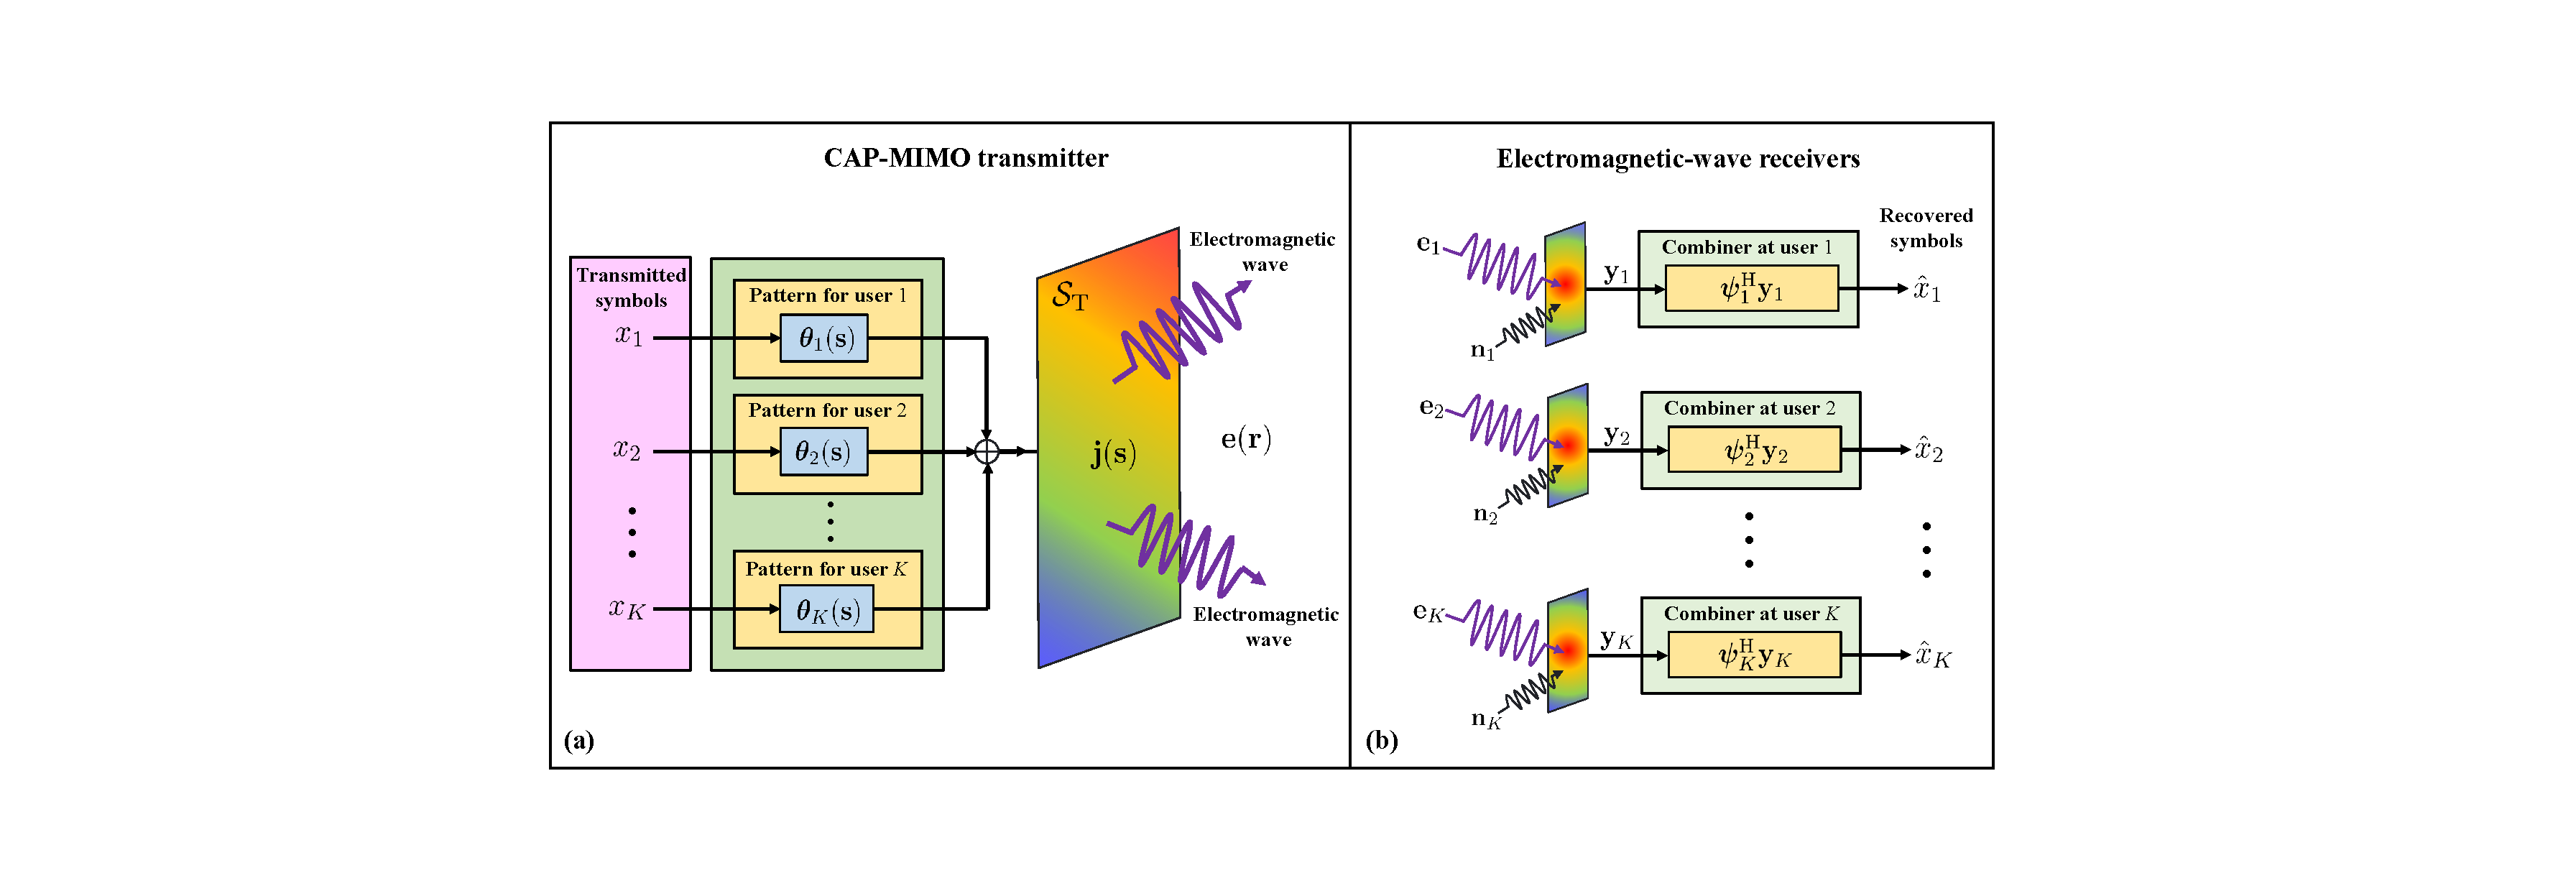
\includegraphics[width=0.85\linewidth]{figures/CAPMIMO.pdf} 
	\caption{Illustration of CAP-MIMO transceivers~\cite{zhang2022pdma}.  }
	\label{fig:CAPMIMO}
\end{figure*}

\subsection{Mutual Information and Capacity Analysis}
Besides the DoF which reveals the number of sub-channels available, the channel capacity is another important performance indicator, which shows the limit of the information transmission rate of the wireless system. Compared to traditional MIMO information theory which uses random vectors as transmitted and received signals, EIT models the EM field as random fields. The random field modeling follows the statistical approach of mutual information and capacity analysis by Shannon. Each realization of the random field represents a pattern of the radiating field. The ensemble of the realizations, to which a probability measure is assigned, depicts the statistical characteristics of the system. 

The mutual information and capacity analysis based on random fields is a continuous extension of the analysis based on random vectors. The main difference between them is that the former approach is in the continuous domain and the latter approach is in the discrete domain. For EIT, the operator theory can be used to represent the autocorrelation properties of the random field. 
Utilizing the Karhunen-Lo\`{e}ve (KL) expansion theorem, the random field can be decomposed into uncorrelated random variables on an orthogonal basis. Then, the continuous channel can be decomposed into parallel sub-channels. Thus, the information obtained from the received random field is evaluated by summing the information over all the sub-channels. 
Different from the matrix determinant form of MIMO information, the EIT information takes a Fredholm determinant form, which is the determinant of an autocorrelation operator. Based on this closed-form Fredholm determinant mutual information formula, the channel capacity of the continuous wireless system can be obtained by maximizing the mutual information over all the possible random field distributions. 



\section{Applications of EIT}
In this section, we introduce several EIT-related applications. 
These technological applications either mimic the analysis methodologies in EIT to fully achieve the existing DoF, or try to explore new communication resources predicted by EIT. 

\subsection{Continuous Aperture MIMO}
Traditional wireless communication systems deploy finite antennas in a limited aperture as the transceivers. 
However, the EIT mutual information analysis is built on spatially continuous theoretical frameworks. 
To bridge the possible gap between the performance limits in MIMO theory and in EIT, CAP-MIMO, which is also called holographic MIMO, is proposed. 
CAP-MIMO adopts a hypothetical structure that contains infinitely dense antennas in a limited spatial region, which is able to continuously generate any current distribution and detect any electric field at the transmitter and the receiver, respectively.  
The current distribution on the transmitter are called patterns of the CAP-MIMO. 
Different signals are modulated onto different patterns before radiated to the space. 
These continuous patterns need to be optimized by specially-designed algorithms in order to achieve a higher multi-user data rate~\cite{zhang2022pdma}. 


% Several works have already explored the pattern design scheme for CAP-MIMO system. The simplest and the easiest way to implement is utilizing the Fourier basis as the patterns, which transfer the approach of OFDM scheme in the time-frequency domain to spatial-wavenumber domain. Other special functions are also utilized to design the patterns in the corresponding assumptions like line-of sight communication or single receiver. For general scenarios, the continuous current patterns can be projected to orthogonal basis and optimization schemes can be utilized to obtain the near-optimal solution of the pattern design scheme.

\subsection{Location Division Multiple Access}
\begin{figure*}[t]
	\centering 
	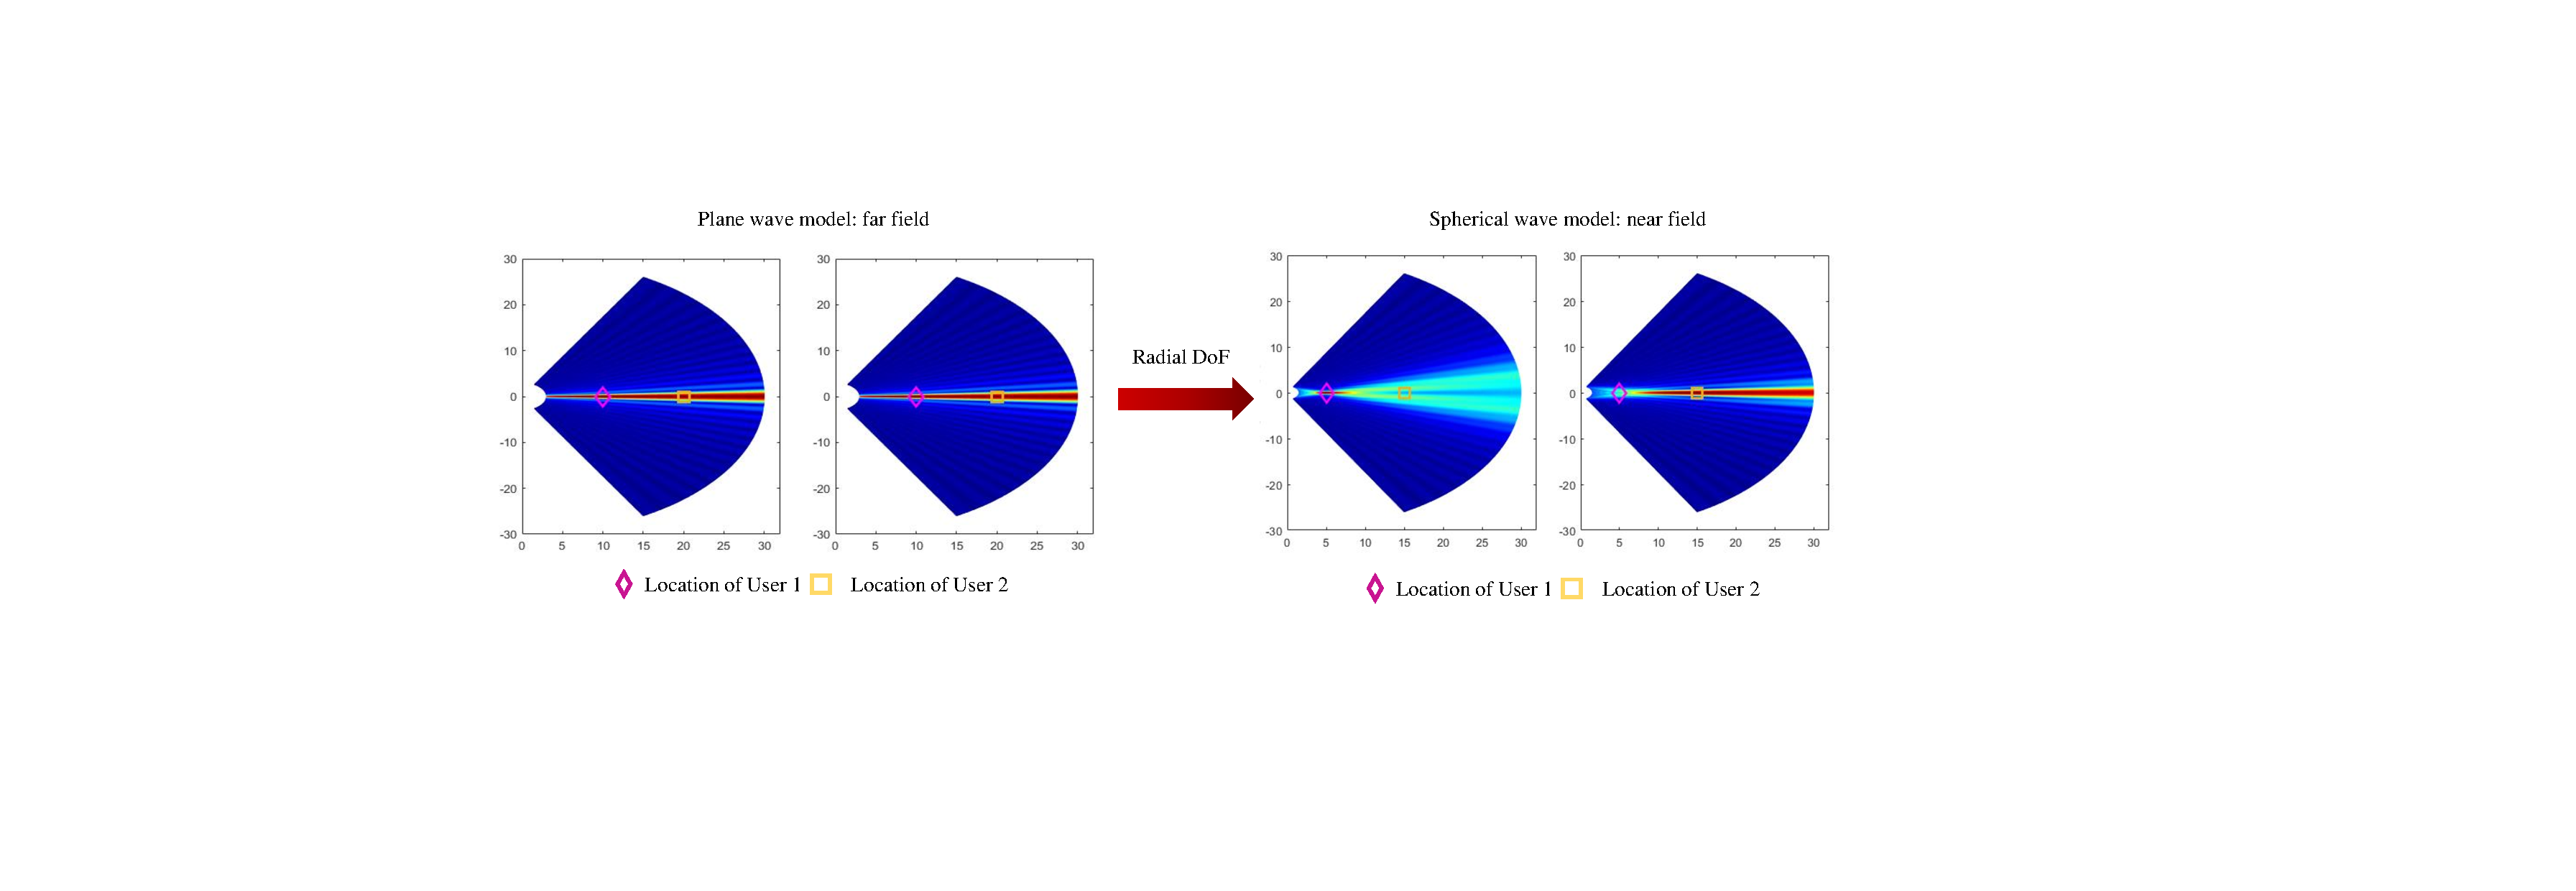
\includegraphics[width=0.9\textwidth]{figures/LDMA.pdf} 
	\caption{Comparison between the SDMA scheme which can not utilize the radial DoF and the LDMA scheme which exploits the radial DoF~\cite{wu2022multiple}. }
	\label{fig:LDMA}
\end{figure*}
For multiple access schemes, the beams emitted from the base station form a functional space. 
The DoF of the functional space represents the resolution of the base station to users at different locations, which corresponds to the analysis of functional DoF in EIT. 	% Relation to the analysis methodologies in EIT. 
Traditional space-division multiple access based on the far-field model can only distinguish the users by the angles and does not utilize the functional DoF in the radial (distance) dimension. 
For massive MIMO systems with large-scale antenna arrays, the spherical wave model is used instead of the planar wave assumption. 
With the spherical wave model, in addition to the angular dimension, the users can also be distinguished along the radial dimension. 
Therefore, a new division scheme called the location division multiple access (LDMA)~\cite{wu2022multiple} is proposed to fully exploit the functional DoF of the beams and serve users at different angles and distances. 
In the LDMA scheme, near-field codebook, beam training, and channel estimation are designed correspondingly, aiming at fully utilizing the spatial resources. 

\subsection{Distance-Aware Precoding}
As discussed in Subsection~\ref{Sec_4_Subsec_1}, the channel DoF of a LoS channel model in EIT is approximately proportional to the length of the transceivers and inversely proportional to the distance between the transceivers. 
Therefore, unlike the traditional far-field scenario which can only support one data stream in the LoS channel model, in the near-field region, the wireless communication system has high channel DoF and can support more than one data stream.
To fully utilize the near-field channel DoF while maintaining low power consumption in the far-field region, a distance-aware precoding scheme is proposed, which adaptively adjusts the number of radio frequency chains to match the channel DoF with different distances.   

% \subsection{Pilot overhead reduction}
% The pilot overhead without channel state information will increase linearly with the number of the antennas. For massive MIMO systems, the pilot overhead will be intolerable. Therefore, to reduce the pilot overhead, the prior information of the channel need to be obtained, which projects the high-dimensional channel matrix on a low-dimensional subspace. Such schemes are actually the expansion of the well-known compressed sensing method, which utilizes the sparsity of the channel. The prior information of the channel can be obtained by building the channel model as a random field and analyzing its statistical characteristics. According to the random channel model, the sparsity of it can be explored to derive the required number of dimensions for channel estimation. 

% \subsection{Field Reconstruction}
% In engineering practice, it is often required to reconstruct the values of an EM field from a finite number of available observations, which is called the field reconstruction problem. 
% To solve this problem, prior information about the EM field is often exploited, including the spatially bandlimited property and the spatial correlation that the EM field possesses. 
% These prior information can be provided by an EIT analysis on the field region. 
% For example, the spatial bandwidth property justifies the cardinal series as asymptotically optimal linear interpolators~\cite{pizzo2022nyquist} of the EM field, while the field correlation methodology leads to Gaussian process regression (GPR)-based field interpolators. 
% These field interpolators are widely applicable to microwave field measurement tasks and channel prediction problems. 


\section{Open Problems}
In this section, we will enumerate some open problems related to EIT, including how to construct a physically compatible noise model, how to specify the power constraint of a continuous-aperture transmitter, how to prove the achievability of the EIT capacity, and what is the fundamental physical limit of manipulating a current density on a continuous transmitting aperture. 

\subsection{Compatible Noise Modeling in Discrete and Continuous Communication Systems}
It can be proved that a purely i.i.d. thermal noise distribution will cause the divergence of the end-to-end capacity of a MIMO transceiver within a constrained aperture size in EIT, when the number of receiving antennas increases indefinitely. 
This is because, as the number of receiving antennas increases, the signals can be aggregated coherently within any small spatial region, while the noises add up out-of-phase because they are uncorrelated. 
Thus, in this small region, the signal energy scales quadratically, while the noise energy scales linearly, leading to an unbounded linear improvement of SNR. Thus, the capacity will diverge to infinity, which is obviously impossible.  

This absurdity is, in fact, caused by the improper assumption that the noise is spatially uncorrelated. 
If we assume a correlated noise, which is possibly the actual correct model, then this capacity divergence naturally disappears. 
As a result, a correlated noise model is needed for the capacity analysis of EIT. This model may be tuned to exhibit a small enough spatial ``coherence length'' to be compatible with the independent MIMO noise model with half a wavelength-spaced antennas, while it does possess some spatial correlation on a small scale to ensure a finite-valued EIT capacity. 
The construction of such a kind of noise model that bridges the macro-scale and micro-scale noises is, up to date, an open problem. 

\subsection{Power Constraint of the Continuous Communication System}
For both classical information theory and EIT, the power constraint is a key factor that affects the mutual information and capacity. 
Therefore, imposing appropriate power constraints on the system is of both theoretical and practical significance. 
In classical information theory, the power constraint is imposed on the expectation of the squared norm of the signal vector.  
Similarly, in EIT, usually the functional L2-norm of the source current is restricted to some pre-determined power value. 
Equivalent expressions of the power constraint in the wavenumber domain can be derived due to the energy-preserving property of the Fourier transform. 

However, some problems are hidden behind such L2 constraint for EIT, among which the most significant one is the incompatibility between the L2 power constraints of MIMO information theory and EM theory.  
In MIMO theory, the signal vectors are complex baseband abstractions of the actual physical process without the guarantee that the squared norm of such vectors represents the actual radiated power. 
However, in EM theory, a more reasonable power constraint is given by calculating the total radiated power from an EM theoretical perspective, rather than calculating the L2-norm of the source current. 
Unfortunately, these two definitions of the power constraint are incompatible and often yield different power values, which is an open problem. 


\subsection{Achievability of the EM Capacity}
In the information theory convention, to establish a ``capacity'' value, one needs to prove an achievability theorem and a converse bound. Only when these two values coincide can one declare that such a value can be called ``capacity''. And usually, the achievability theorem is relatively more difficult, which requires ingenious mathematical constructions~\cite{shannon1948mathematical}. 

The EIT capacity, though carefully defined in~\cite{wan2022mutual,zhang2022pdma}, is far from perfection, since they all lack an achievability proof. 
To prove the achievability of such EM capacity, following Shannon's stochastic proof techniques, a spatio-temporal waveform-based channel codebook may be constructed, which deserves further research and rigorous mathematical construction.  

\subsection{Physical Granuarity Limit of the Current Manipulation and Electric Field Detection}
In the current research on EIT, most works assume that the EM field is arbitrarily adjustable and detectable. From another perspective, this assumption can be viewed as placing an infinite number of antennas in the source and destination regions that can work without interference. However, practical communication systems cannot fulfill such infinite granuarity requirements. In fact, antenna mutual coupling effects always exists because of imperfect antenna isolation. Considering the mutual coupling of the antennas, we cannot fabricate an infinitely dense antenna array, which means that the current manipulation and electric field detection of practical systems are all subject to a limited accuracy. To guide the design of practical systems, the physical limit of the current manipulation and electric field detection remains to be explored. 

\section{Conclusions}
In this paper, to reveal the fundamental physical limit of wireless information transmission imposed by the underlying EM mechanisms, we have thoroughly investigated the basic concepts, mathematical tools, modeling methodologies, and information-theoretic analyses that constitute the EIT. 
Furthermore, we have briefly reviewed the novel applications related to EIT, aiming at designing new wireless communication systems for capacity enhancement and accessibility improvement. Though recent progress on EIT demonstrates its possibility to become a unified and widely-applicable theory, there are still some unresolved issues that may cause confusion, including the incompatibility of EIT with existing MIMO theory, the unknown hidden physical constraints that influence the sampling density, and the immature proofs of information-theoretic achievability and converse bounds in EIT. % insights added here. 
To address these problems, a special relativity-based electromagnetic theory that exhibits more symmetries may be introduced into the study of EIT to facilitate theoretic analysis.  


\footnotesize

\bibliographystyle{IEEEtran}
\bibliography{EIT, IEEEabrv}

\normalsize
\section*{Biographies}

{\bf Jieao Zhu} is a Ph.D. researcher in BNRist from Tsinghua University, Beijing, China.
\\

{\bf Zhongzhichao Wan} is a Ph.D. researcher in BNRist from Tsinghua University, Beijing, China.
\\


{\bf Linglong Dai} is an associate professor at Tsinghua University. He has received six conference best paper awards and four journal best paper awards. 


\end{document}


